\documentclass{beamer}
\usepackage{amsfonts,amsmath,oldgerm}
\usepackage{tabularx, booktabs, multirow, siunitx}
\usetheme{sintef}

\newcommand{\testcolor}[1]{\colorbox{#1}{\textcolor{#1}{test}}~\texttt{#1}}

\usefonttheme[onlymath]{serif}

\titlebackground*{assets/background}

\newcommand{\hrefcol}[2]{\textcolor{cyan}{\href{#1}{#2}}}

\title{TinyViT: A Small Vision Transformer}
\course{Master's Degree in Computer Science}
\author{\href{mailto:crainic1938430@studenti.uniroma1.it}{Lucian Dorin Crainic}}
\IDnumber{1938430}
\date{Academic Year 2024/2025}

\begin{document}
\maketitle

\begin{frame}

  This project is based on the well known \textbf{Vision Transformer} (ViT) architecture, a deep learning model that applies self attention mechanisms to image processing. We will start by introducing the core principles of ViT, explaining how it differs from traditional CNNs.

  \vspace{\baselineskip}

  Then, we will explore the \textbf{TinyViT} a smaller implementation of the ViT architecture. Finally, we will present benchmark results demonstrating its performance across various tasks.

\end{frame}

\section{Introduction}

Transformers, introduced by \cite{vaswani2017attention} for natural language processing (NLP), have become the dominant architecture for sequence modeling due to their scalability and self-attention mechanisms. Inspired by their success in NLP, \cite{alexey2020image} pioneered the Vision Transformer (ViT), demonstrating that transformers can achieve state-of-the-art results in image recognition by treating images as sequences of patch tokens. By splitting an image into fixed-size patches, linearly embedding them, and processing the sequence with a standard transformer encoder, ViT outperformed convolutional neural networks (CNNs) \cite{he2016deep} on large-scale datasets like ImageNet when pretrained on massive datasets (e.g., JFT-300M). However, ViT’s strong performance comes at a cost: it requires extensive computational resources and large pretraining datasets, raising practical barriers for adoption in settings where such infrastructure is unavailable.

In this work, we aim to (1) elucidate the foundational mechanics of Vision Transformers and (2) present TinyViT, a minimalist implementation designed to test the viability of ViTs in simplified, resource-efficient settings. Unlike the original ViT, which emphasizes scaling to massive datasets, TinyViT reduces architectural complexity—employing fewer transformer layers, smaller embedding dimensions, and streamlined attention mechanisms—while retaining the core principles of patch-based processing and self-attention. We evaluate TinyViT on widely adopted benchmarks like CIFAR-10 and CIFAR-100 \cite{krizhevsky2009learning}, and STL-10 \cite{coates2011analysis}, datasets that reflect real-world scenarios where data and computational resources are often constrained.
\section{Vision Transformer}

\begin{frame}[fragile]{Vision Transformer Architecture}
  \framesubtitle{Patch Embedding and Positional Econding}
  \textbf{Patch Embedding:}
  \begin{itemize}
    \item Converts images into \textbf{fixed size patches}.
    \item Each patch is flattened into a vector and projected into an \textbf{embedding space}.
      \begin{equation}
        X \in \mathbb{R}^{H \times W \times C} \quad \Rightarrow \quad N = \frac{H \times W}{P^2}
      \end{equation}
      \begin{equation}
        Z = [z_1, z_2, ..., z_N] \in \mathbb{R}^{N \times D}
      \end{equation}
  \end{itemize}

  \textbf{Positional Encoding:}
  \begin{itemize}
    \item Adds \textbf{spatial information} to the patches since transformers lack inherent \textbf{spatial bias}.
    \item Learnable positional embeddings:
      \begin{equation}
        Z_0 = Z + E_{pos}
      \end{equation}
  \end{itemize}
\end{frame}

\begin{frame}[fragile]{Vision Transformer Architecture}
  \framesubtitle{Transformer Encoder and Classification Head}
  \textbf{Transformer Encoder:}
  \begin{itemize}
    \item Processes the \textbf{sequence} of patch embeddings.
    \item Consists of multiple layers of \textbf{Multi Head Self Attention} (\textit{MHSA}) and \textbf{Feed Forward Networks} (\textit{FFN}).
      \begin{equation}
        Q = Z W_Q, \quad K = Z W_K, \quad V = Z W_V
      \end{equation}
      \begin{equation}
        \text{Attention}(Q, K, V) = \text{softmax} \left( \frac{QK^T}{\sqrt{d}} \right) V
      \end{equation}
      \begin{equation}
        FFN(z) = \text{GELU} (zW_1 + b_1) W_2 + b_2
      \end{equation}
    \end{itemize}

  \textbf{Classification Head:}
  \begin{itemize}
    \item Uses the class token $ z_{cls} $ for \textbf{final classification}.
    \item \textbf{Softmax layer} for output prediction:
      \begin{equation}
        \hat{y} = \text{softmax} (W_c z_{cls} + b_c)
      \end{equation}
  \end{itemize}
\end{frame}

\begin{frame}[fragile]{ViT vs. CNN}
  \framesubtitle{A brief comparision between the two models}
  \begin{columns}
    \begin{column}{\textwidth}
      \begin{itemize}
        \item CNNs use \textbf{convolutional layers} with local receptive fields.
        \item ViTs process images globally using \textbf{self attention} mechanisms.
        \item CNNs have built in \textbf{spatial hierarchies}, whereas ViTs rely on attention.
        \item ViTs typically need \textbf{more data} to perform well but can model long range dependencies.
      \end{itemize}
    \end{column}
  \end{columns}
  \begin{figure}
    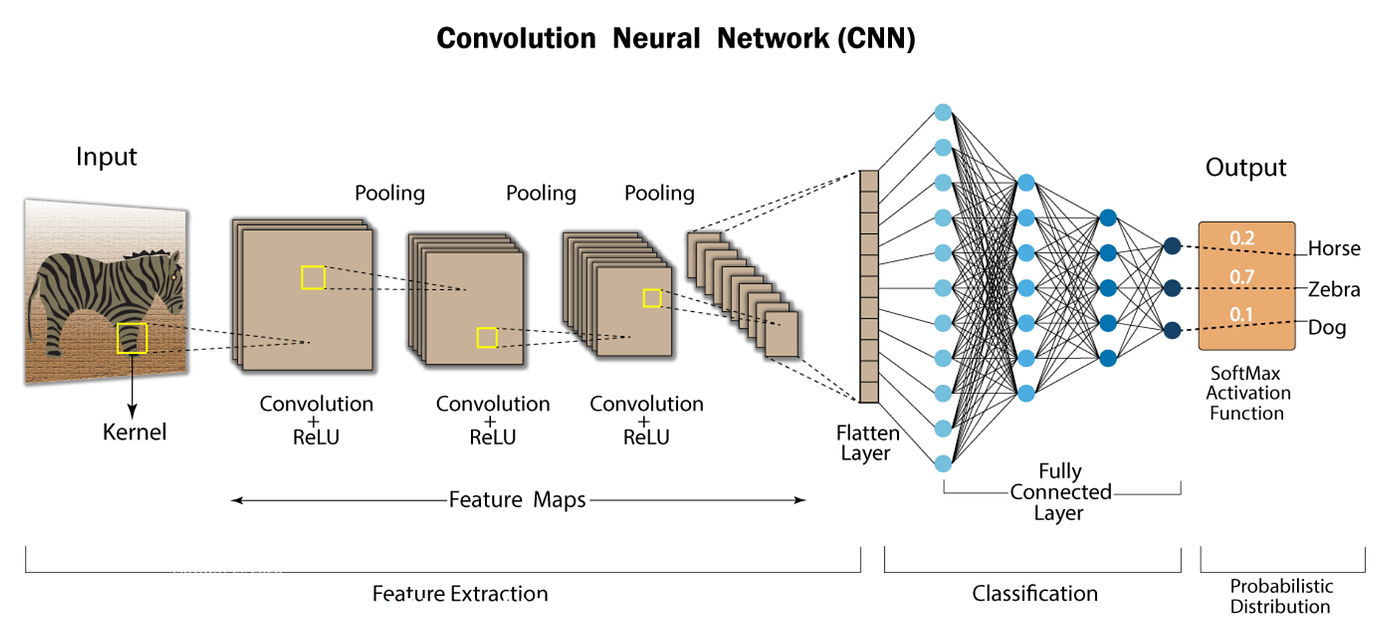
\includegraphics[width=0.6\textwidth]{images/cnn_architecture.png}
  \end{figure}
\end{frame}
\section{TinyViT}

\begin{sidepic}{./images/code.png}{TinyViT Architecture}
  \framesubtitle{Our tiny model}
  \begin{itemize}
    \item A minimal Vision Transformer designed for smaller datasets.
    \item Reduces architectural complexity while preserving key transformer principles.
    \item Uses fewer layers, smaller embedding dimensions, and computationally efficient components.
  \end{itemize}
\end{sidepic}

\begin{frame}[fragile]{TinyViT Parameters}
  \framesubtitle{What parameters do we use ?}
  \begin{table}[htbp]
    \small
    \centering
    \caption{Parameters of the TinyViT Model for CIFAR-10}
    \begin{tabular}{@{}ll@{}}
      \toprule
      \textbf{Parameter} & \textbf{Value} \\
      \midrule
      Number of Classes & 10 \\
      Embedding Dimension & 128 \\
      Image Size & 32 \\
      Patch Size & 4 \\
      Input Channels & 3 \\
      Number of Attention Heads & 8 \\
      Number of Transformer Layers & 6 \\
      MLP Hidden Dimension & 512 \\
      \bottomrule
    \end{tabular}
  \end{table}
\end{frame}

\begin{frame}{Differences between TinyViT and ViT}
  \framesubtitle{Some differences between the two models}
  \begin{itemize}
    \item TinyViT has significantly fewer transformer layers than standard ViT.
    \item Smaller embedding dimensions to reduce computational costs.
    \item Optimized for smaller datasets, unlike ViT, which requires large-scale pretraining.
    \item Lower memory footprint, making it feasible for resource-constrained environments.
  \end{itemize}
\end{frame}
\section{Dataset}


\section{Training Setup}
\begin{frame}{Models Training Setup}
    Compared to PowerPoint, using \LaTeX\ is better because:
    \begin{itemize}
    \item \textbf{Optimizer} : AdamW
    \item \textbf{Learning Rate} : AdamW
    \item \textbf{Weight Decay} : AdamW
    \item \textbf{Loss Function} : AdamW
    \item \textbf{Epochs} : AdamW
    \item \textbf{Batch Size} : AdamW
    \end{itemize}
\end{frame}
\section{Evaluation Metrics}


\section{Conlusions and Future Work}

\begin{frame}{Conclusion}
  \begin{itemize}
    \item TinyViT proves that \textbf{transformer based models} can be efficient with fewer resources.
    \item Outperforms CNNs on \textbf{smaller datasets} like CIFAR-10 and CIFAR-100.
    \item \textbf{Requires improvements} for larger images like STL-10.
  \end{itemize}
\end{frame}

\begin{frame}[fragile]{Future Work}
  \begin{columns}
    \begin{column}{0.7\textwidth}
      \begin{itemize}
        \item Implement TinyViT for \textbf{Object Detection} (DETR) and \textbf{Segmentation} (Segmenter).
        \item Experiment with different \textbf{hyperparameters} (layers, embedding size, attention heads).
        \item Explore pretraining on \textbf{larger datasets} to improve performance.
      \end{itemize}
    \end{column}
    \begin{column}{0.3\textwidth}
      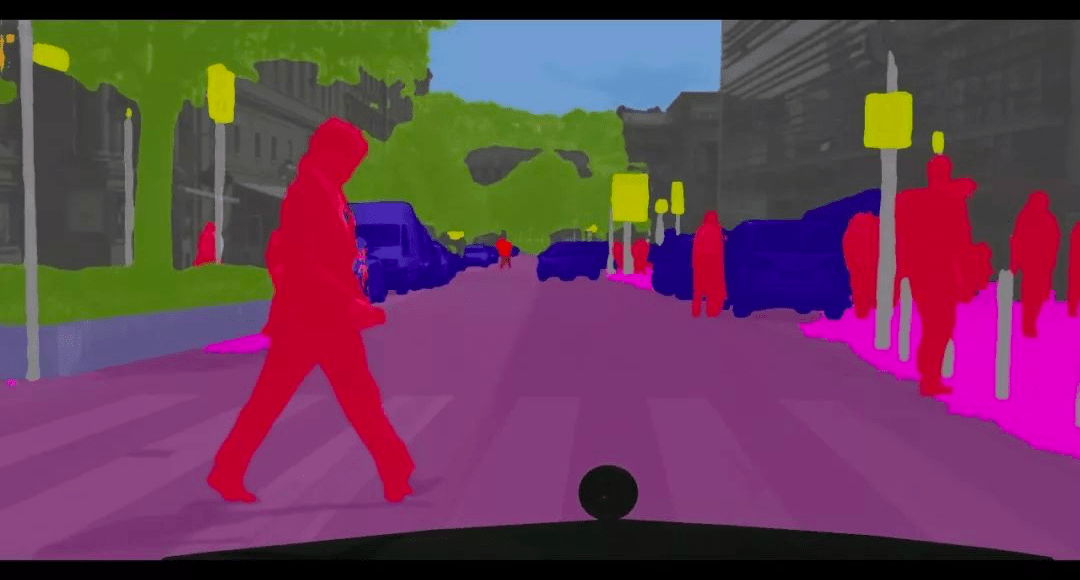
\includegraphics[width=\textwidth]{images/segmentation.png}
      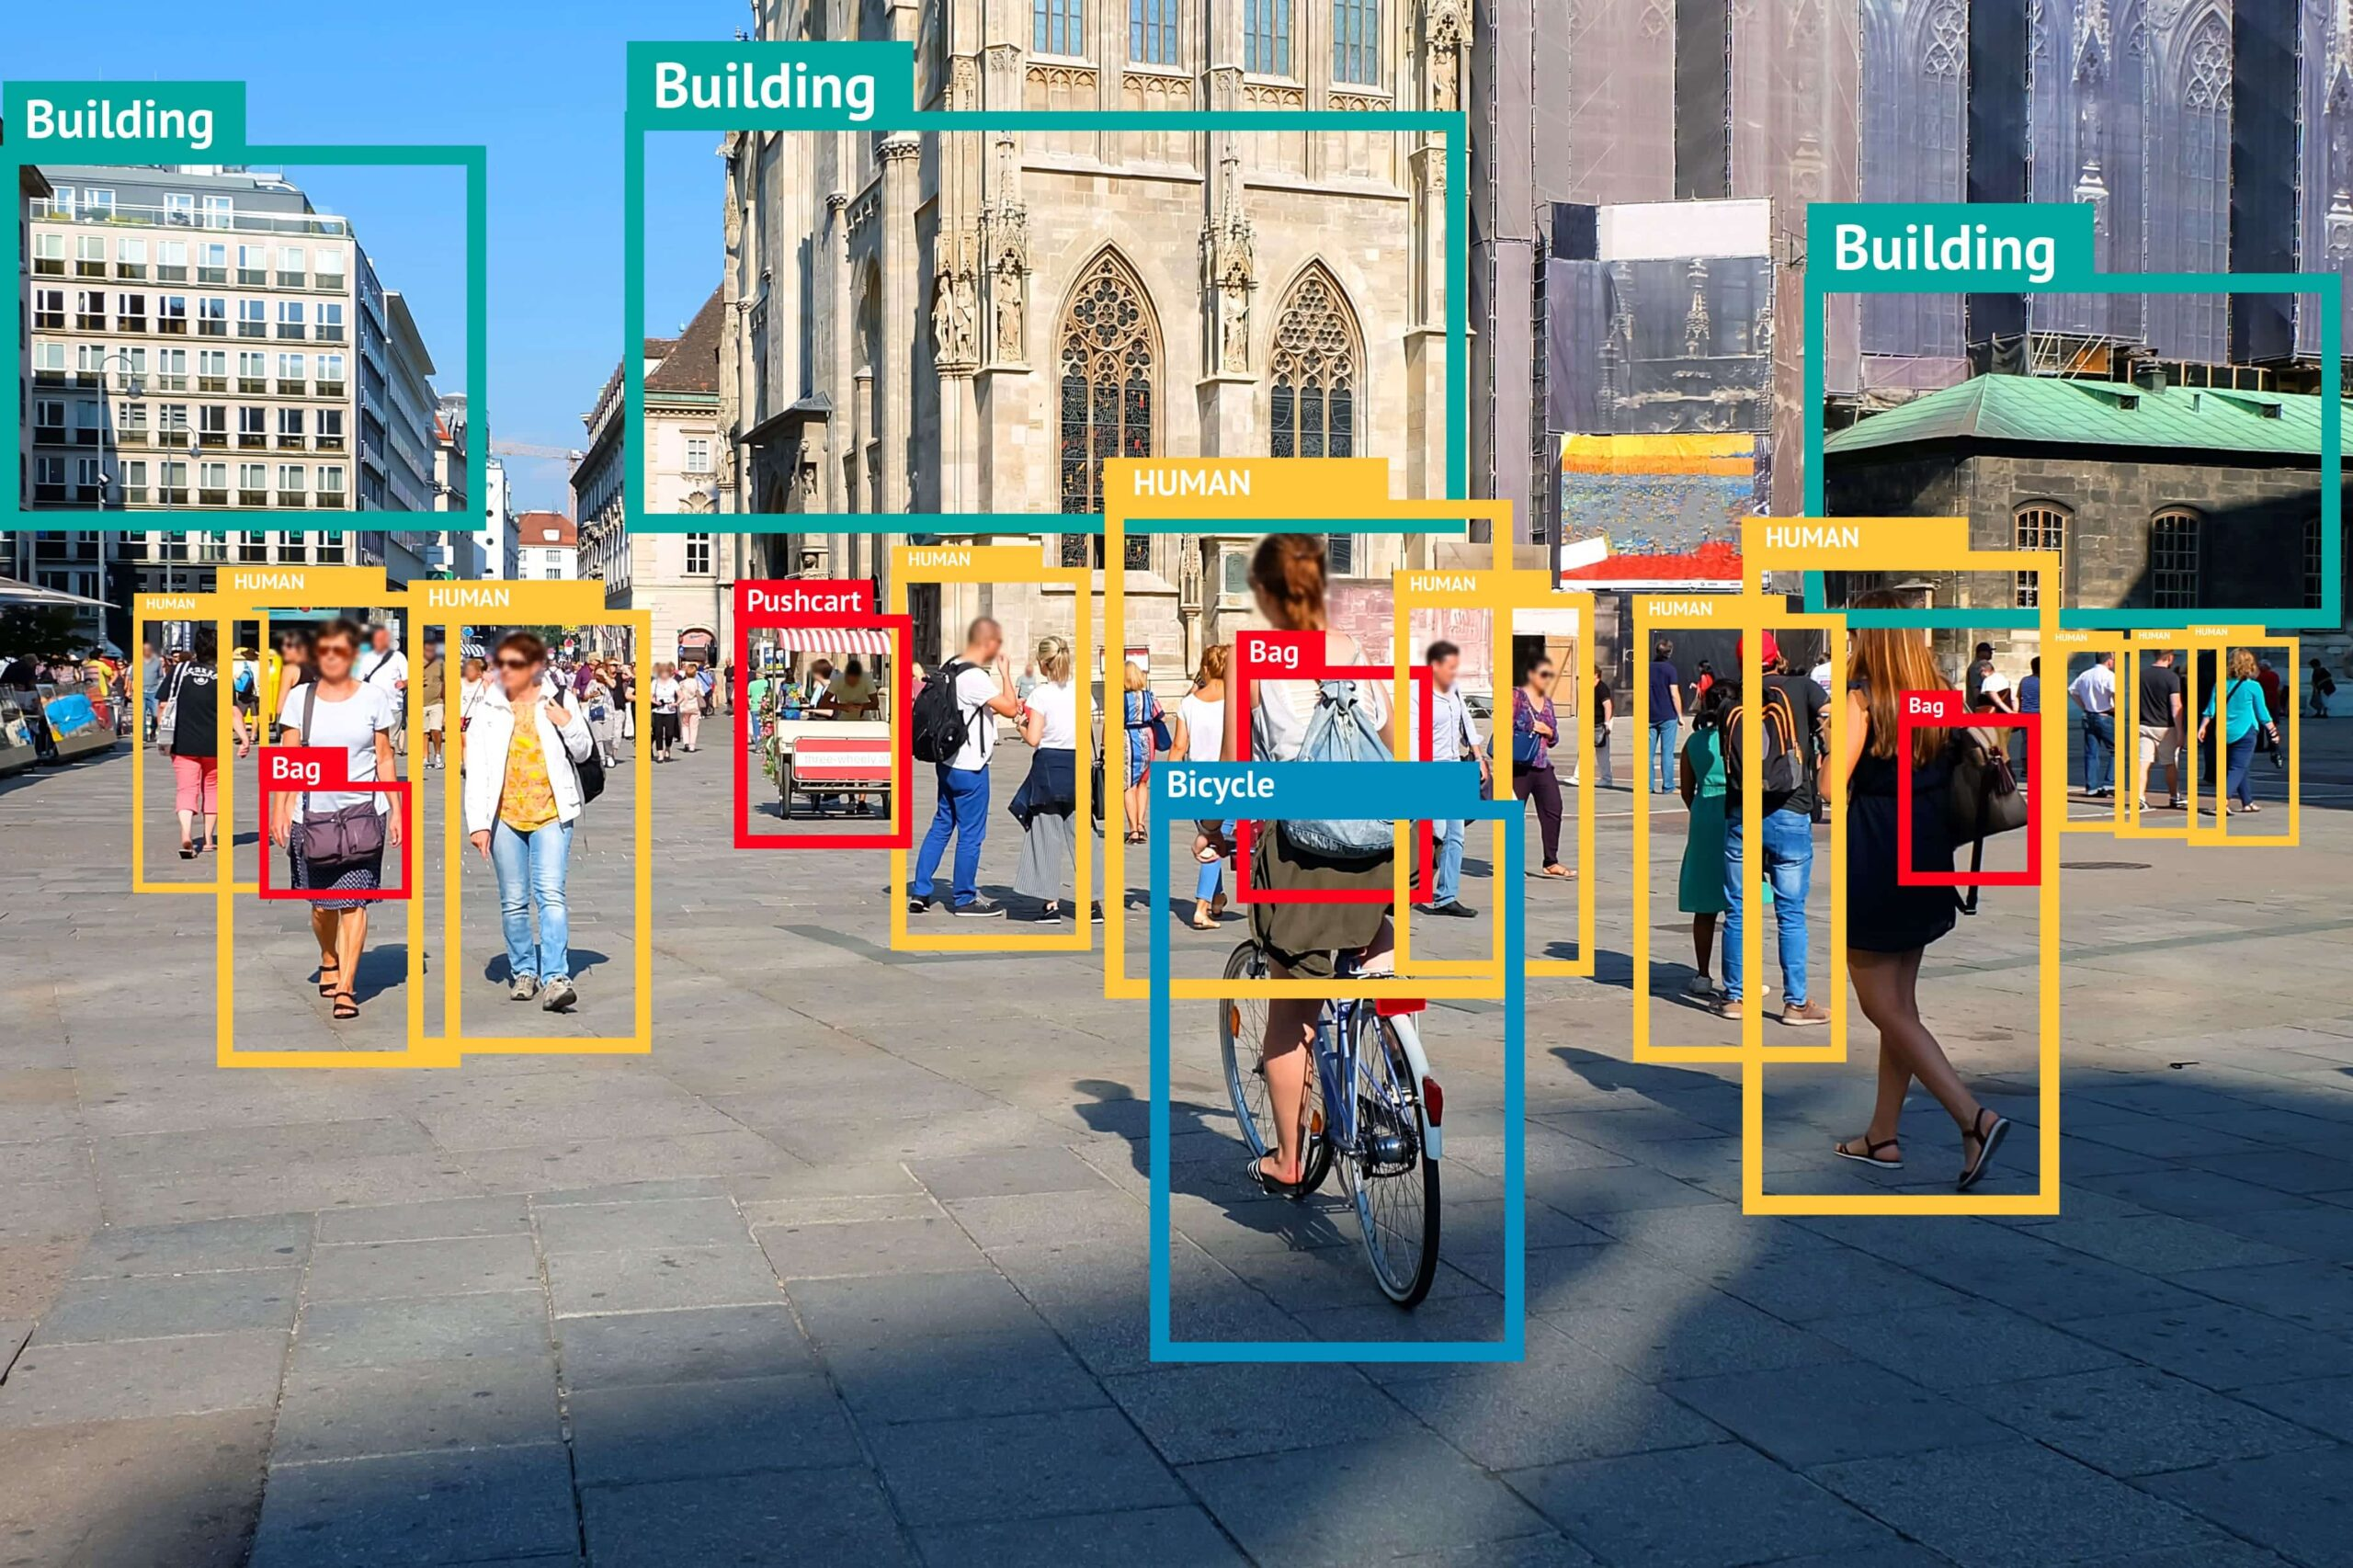
\includegraphics[width=\textwidth]{images/objectdetection.jpg}
    \end{column}
  \end{columns}
\end{frame}

\backmatter

\end{document}